\pgfdeclarelayer{background}
\pgfsetlayers{background,main}

\colorlet{circle edge}{black!50}
\colorlet{circle area}{gray!20}

\def\SourceSink{{(0, 3)/s}, {(0.5, 0)/t}}
\def\network{{(0.2, 2.6)/-}, {(0.9, 2.4)/a}, {(-0.6, 2.3)/b}, {(0.3, 2)/c}, {(-1.1, 2.2)/d}, {(-0.1, 1.4)/e}, {(0.9, 1.6)/f}, {(-1.2, 1.4)/g}, {(0.2, 0.5)/h}, {(-0.7, 1.8)/i}, {(-0.9, 1)/j}, {(-0.5, 0.8)/k}, {(-0.3, 0.3)/l}}
\def\moveNodePos{(0.3, 1)}
\def\connect{s/-, -/a, a/c, c/-, a/f, c/f, c/e, e/i, i/b, i/d, d/b, b/-, i/g, g/j, j/k, k/l, l/h, h/t}
\def\connectExtra{e/*, */h}
\def\backgroundConnectOne{s/-, -/c, c/e, e/*, */h, h/t}
\def\backgroundConnectTwo{s/-, -/c, c/e}

\tikzset{
  filled/.style={fill=circle area, draw=circle edge, thick},
  outline/.style={draw=circle edge, thick},
  dash/.style={very thick, dashed}    
  }

\setlength{\parskip}{5mm}

\tikzstyle{edge} = [draw, thick, -]
\tikzstyle{vertex}=[circle,fill=black!50,minimum size=10pt,inner sep=0pt]
\tikzstyle{invis-vertex}=[circle,fill=white!100,minimum size=0pt, inner sep=0pt]

\tikzstyle{selected edge} = [draw, line width=5pt,-,gray!50]
\tikzstyle{edge} = [draw, thick, -]

\subfloat[Initial]{\label{fig:changed_route1}
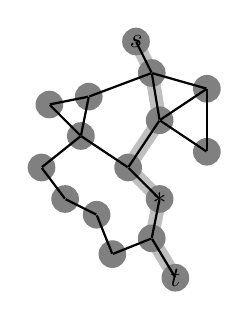
\begin{tikzpicture} 
  % The source and the sink, and the new node
  \foreach \pos/\name in \SourceSink {
    \node[invis-vertex] (\name) at \pos {};
    \node[vertex] () at \pos {$\name$};
    }
       
   \node[invis-vertex] (*) at \moveNodePos {};
   \node[vertex] () at \moveNodePos {$*$};
        
   % The rest of the nodes
   \foreach \pos/\name in \network {
     \node[invis-vertex] (\name) at \pos {};
     \node[vertex] () at \pos {};
     } 

   % Background layer
   \begin{pgfonlayer}{background}
     \foreach \source/ \dest in \backgroundConnectOne {
       \path[selected edge] (\source) -- (\dest);
       }
   \end{pgfonlayer}

   % All the connections but the ones to *
   \foreach \source/\sink in \connect {
     \path[edge] (\source) -- (\sink);
     }
       
   \foreach \source/\sink in \connectExtra {
     \path[edge] (\source) -- (\sink);
     }
\end{tikzpicture}}
% Remove empty line
\subfloat[Node $*$ has moved away]{\label{fig:changed_route2}
\begin{tikzpicture} 
  % The source and the sink, and the new node
  \foreach \pos/\name in \SourceSink {
    \node[vertex] (\name) at \pos {$\name$};
    }
 
  \draw[dash] {\moveNodePos circle (5pt)} {};
        
  % The rest of the nodes
  \foreach \pos/\name in \network
    \node[vertex] (\name) at \pos {}; 

  % Background layer
  \begin{pgfonlayer}{background}
    \foreach \source/ \dest in \backgroundConnectTwo
      \path[selected edge] (\source) -- (\dest);
  \end{pgfonlayer}

  % All the connections but the ones to *
  \foreach \source/\sink in \connect
    \path[edge] (\source) -- (\sink);
\end{tikzpicture}}
